\hypertarget{Utils_8h}{
\section{Utils.h File Reference}
\label{Utils_8h}\index{Utils.h@{Utils.h}}
}


This graph shows which files directly or indirectly include this file:\begin{figure}[H]
\begin{center}
\leavevmode
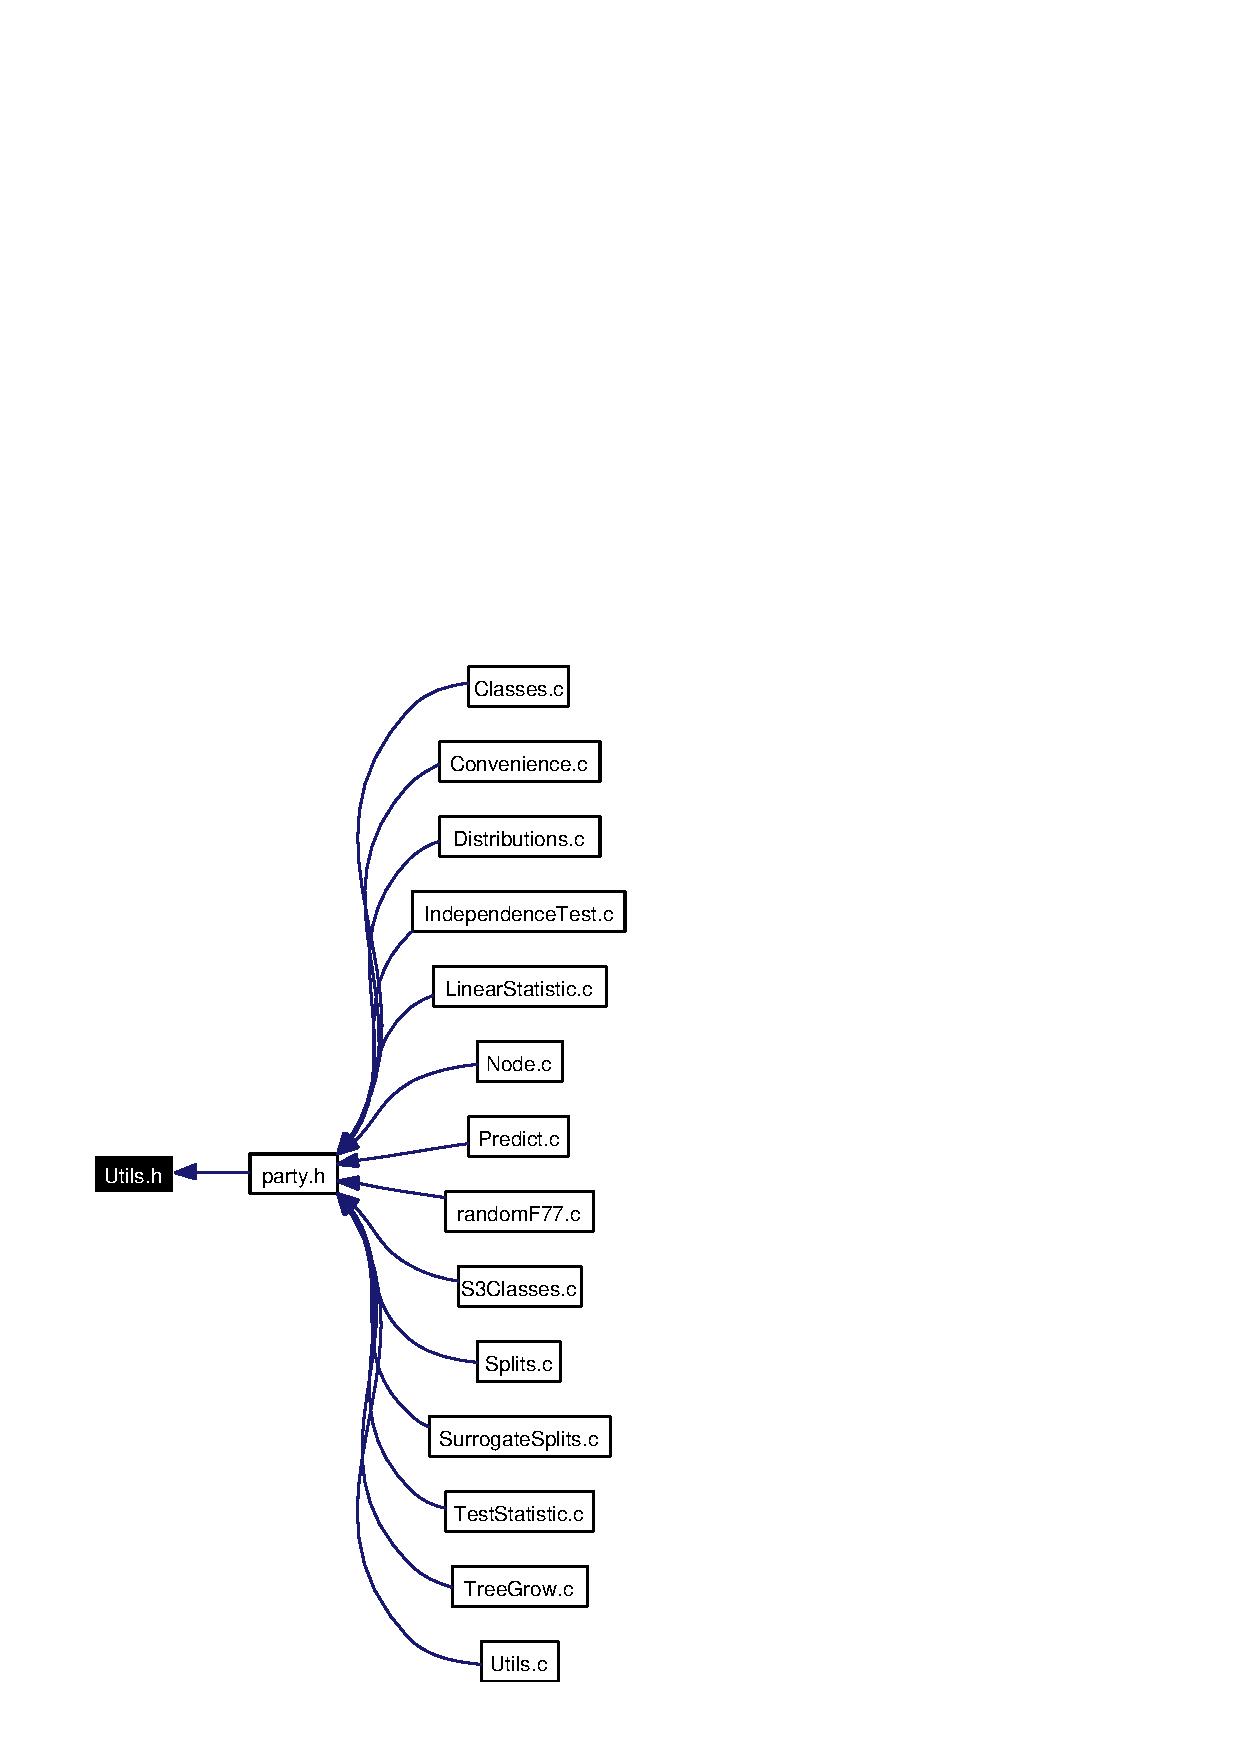
\includegraphics[width=153pt]{Utils_8h__dep__incl}
\end{center}
\end{figure}
\subsection*{Functions}
\begin{CompactItemize}
\item 
void \hyperlink{Utils_8h_a0}{C\_\-kronecker} (const double $\ast$A, const int m, const int n, const double $\ast$B, const int r, const int s, double $\ast$ans)
\item 
SEXP \hyperlink{Utils_8h_a1}{La\_\-svd} (SEXP jobu, SEXP jobv, SEXP x, SEXP s, SEXP u, SEXP v, SEXP method)
\item 
void \hyperlink{Utils_8h_a2}{C\_\-Sample\-No\-Replace} (int $\ast$x, int m, int k, int $\ast$ans)
\item 
void \hyperlink{Utils_8h_a3}{C\_\-MPinv} (SEXP x, double tol, SEXP svdmem, SEXP ans)
\item 
double \hyperlink{Utils_8h_a4}{C\_\-max} (const double $\ast$x, const int n)
\item 
void \hyperlink{Utils_8h_a5}{C\_\-abs} (double $\ast$x, int n)
\item 
void \hyperlink{Utils_8h_a6}{C\_\-matprod} (double $\ast$x, int nrx, int ncx, double $\ast$y, int nry, int ncy, double $\ast$z)
\item 
void \hyperlink{Utils_8h_a7}{C\_\-matprod\-T} (double $\ast$x, int nrx, int ncx, double $\ast$y, int nry, int ncy, double $\ast$z)
\item 
int \hyperlink{Utils_8h_a8}{nrow} (SEXP x)
\item 
int \hyperlink{Utils_8h_a9}{ncol} (SEXP y)
\item 
int \hyperlink{Utils_8h_a10}{C\_\-whichmax} (double $\ast$pvalue, double $\ast$teststat, int ninputs)
\item 
int \hyperlink{Utils_8h_a11}{i\_\-in\_\-set} (int i, int $\ast$iset, int p)
\item 
int \hyperlink{Utils_8h_a12}{C\_\-i\_\-in\_\-set} (int i, SEXP set)
\end{CompactItemize}


\subsection{Function Documentation}
\hypertarget{Utils_8h_a5}{
\index{Utils.h@{Utils.h}!C_abs@{C\_\-abs}}
\index{C_abs@{C\_\-abs}!Utils.h@{Utils.h}}
\subsubsection[C\_\-abs]{\setlength{\rightskip}{0pt plus 5cm}void C\_\-abs (double $\ast$ {\em x}, int {\em n})}}
\label{Utils_8h_a5}


absolute value \begin{Desc}
\item[Parameters:]
\begin{description}
\item[{\em x}]numeric vector \item[{\em n}]length(x)\end{description}
\end{Desc}


Definition at line 259 of file Utils.c.

Referenced by C\_\-absstandardize(), and R\_\-abs().\hypertarget{Utils_8h_a12}{
\index{Utils.h@{Utils.h}!C_i_in_set@{C\_\-i\_\-in\_\-set}}
\index{C_i_in_set@{C\_\-i\_\-in\_\-set}!Utils.h@{Utils.h}}
\subsubsection[C\_\-i\_\-in\_\-set]{\setlength{\rightskip}{0pt plus 5cm}int C\_\-i\_\-in\_\-set (int {\em i}, SEXP {\em set})}}
\label{Utils_8h_a12}




Definition at line 473 of file Utils.c.

References i\_\-in\_\-set().

Referenced by C\_\-get\_\-node().

Here is the call graph for this function:\begin{figure}[H]
\begin{center}
\leavevmode
\includegraphics[width=94pt]{Utils_8h_a12_cgraph}
\end{center}
\end{figure}
\hypertarget{Utils_8h_a0}{
\index{Utils.h@{Utils.h}!C_kronecker@{C\_\-kronecker}}
\index{C_kronecker@{C\_\-kronecker}!Utils.h@{Utils.h}}
\subsubsection[C\_\-kronecker]{\setlength{\rightskip}{0pt plus 5cm}void C\_\-kronecker (const double $\ast$ {\em A}, const int {\em m}, const int {\em n}, const double $\ast$ {\em B}, const int {\em r}, const int {\em s}, double $\ast$ {\em ans})}}
\label{Utils_8h_a0}


Computes the Kronecker product of two matrices\par
 \begin{Desc}
\item[Parameters:]
\begin{description}
\item[{\em A}]matrix \item[{\em m}]nrow(A) \item[{\em n}]ncol(A) \item[{\em B}]matrix \item[{\em r}]nrow(B) \item[{\em s}]ncol(B) \item[{\em ans}]return value; a pointer to a REALSXP-vector of length (mr x ns)\end{description}
\end{Desc}


Definition at line 23 of file Utils.c.

Referenced by C\_\-Expect\-Covar\-Linear\-Statistic(), and R\_\-kronecker().\hypertarget{Utils_8h_a6}{
\index{Utils.h@{Utils.h}!C_matprod@{C\_\-matprod}}
\index{C_matprod@{C\_\-matprod}!Utils.h@{Utils.h}}
\subsubsection[C\_\-matprod]{\setlength{\rightskip}{0pt plus 5cm}void C\_\-matprod (double $\ast$ {\em x}, int {\em nrx}, int {\em ncx}, double $\ast$ {\em y}, int {\em nry}, int {\em ncy}, double $\ast$ {\em z})}}
\label{Utils_8h_a6}


matrix product x $\ast$\% y \begin{Desc}
\item[Parameters:]
\begin{description}
\item[{\em x}]a matrix \item[{\em nrx}]number of rows of x \item[{\em ncx}]number of cols of x \item[{\em y}]a matrix \item[{\em nry}]number of rows of y \item[{\em ncy}]number of cols of y \item[{\em z}]a matrix of dimension nrx x ncy\end{description}
\end{Desc}


Definition at line 297 of file Utils.c.

Referenced by C\_\-MLinear\-Statistic(), R\_\-matprod(), and R\_\-predict\-RF2().\hypertarget{Utils_8h_a7}{
\index{Utils.h@{Utils.h}!C_matprodT@{C\_\-matprodT}}
\index{C_matprodT@{C\_\-matprodT}!Utils.h@{Utils.h}}
\subsubsection[C\_\-matprodT]{\setlength{\rightskip}{0pt plus 5cm}void C\_\-matprod\-T (double $\ast$ {\em x}, int {\em nrx}, int {\em ncx}, double $\ast$ {\em y}, int {\em nry}, int {\em ncy}, double $\ast$ {\em z})}}
\label{Utils_8h_a7}


matrix product x $\ast$\% t(y) \begin{Desc}
\item[Parameters:]
\begin{description}
\item[{\em x}]a matrix \item[{\em nrx}]number of rows of x \item[{\em ncx}]number of cols of x \item[{\em y}]a matrix \item[{\em nry}]number of rows of y \item[{\em ncy}]number of cols of y \item[{\em z}]a matrix of dimension nrx x ncy\end{description}
\end{Desc}


Definition at line 349 of file Utils.c.

Referenced by C\_\-MLinear\-Statistic(), and R\_\-matprod\-T().\hypertarget{Utils_8h_a4}{
\index{Utils.h@{Utils.h}!C_max@{C\_\-max}}
\index{C_max@{C\_\-max}!Utils.h@{Utils.h}}
\subsubsection[C\_\-max]{\setlength{\rightskip}{0pt plus 5cm}double C\_\-max (const double $\ast$ {\em x}, const int {\em n})}}
\label{Utils_8h_a4}


the maximum of a double vector \begin{Desc}
\item[Parameters:]
\begin{description}
\item[{\em x}]vector \item[{\em n}]its length\end{description}
\end{Desc}


Definition at line 222 of file Utils.c.

Referenced by C\_\-maxabs\-Test\-Statistic(), C\_\-Monte\-Carlo(), C\_\-Node(), and R\_\-max().\hypertarget{Utils_8h_a3}{
\index{Utils.h@{Utils.h}!C_MPinv@{C\_\-MPinv}}
\index{C_MPinv@{C\_\-MPinv}!Utils.h@{Utils.h}}
\subsubsection[C\_\-MPinv]{\setlength{\rightskip}{0pt plus 5cm}void C\_\-MPinv (SEXP {\em x}, double {\em tol}, SEXP {\em svdmem}, SEXP {\em ans})}}
\label{Utils_8h_a3}


Moore-Penrose inverse of a matrix \begin{Desc}
\item[Parameters:]
\begin{description}
\item[{\em x}]matrix \item[{\em tol}]a tolerance bound \item[{\em svdmem}]an object of class `svd\_\-mem' \item[{\em ans}]return value; an object of class `Expect\-Covar\-MPinv'\end{description}
\end{Desc}


Definition at line 128 of file Utils.c.

References CR\_\-svd(), PL2\_\-MPinv\-Sym, PL2\_\-rank\-Sym, and PL2\_\-svd\-Sym.

Referenced by C\_\-Lin\-Stat\-Exp\-Cov\-MPinv(), and R\_\-MPinv().

Here is the call graph for this function:\begin{figure}[H]
\begin{center}
\leavevmode
\includegraphics[width=134pt]{Utils_8h_a3_cgraph}
\end{center}
\end{figure}
\hypertarget{Utils_8h_a2}{
\index{Utils.h@{Utils.h}!C_SampleNoReplace@{C\_\-SampleNoReplace}}
\index{C_SampleNoReplace@{C\_\-SampleNoReplace}!Utils.h@{Utils.h}}
\subsubsection[C\_\-SampleNoReplace]{\setlength{\rightskip}{0pt plus 5cm}void C\_\-Sample\-No\-Replace (int $\ast$ {\em x}, int {\em m}, int {\em k}, int $\ast$ {\em ans})}}
\label{Utils_8h_a2}


compute a permutation of a (random subset of) 0:(m-1) \begin{Desc}
\item[Parameters:]
\begin{description}
\item[{\em x}]an integer vector of length m \item[{\em m}]integer \item[{\em k}]integer \item[{\em ans}]an integer vector of length k\end{description}
\end{Desc}


Definition at line 397 of file Utils.c.

Referenced by C\_\-Global\-Test(), C\_\-Monte\-Carlo(), R\_\-Ensemble(), R\_\-permute(), and R\_\-rsubset().\hypertarget{Utils_8h_a10}{
\index{Utils.h@{Utils.h}!C_whichmax@{C\_\-whichmax}}
\index{C_whichmax@{C\_\-whichmax}!Utils.h@{Utils.h}}
\subsubsection[C\_\-whichmax]{\setlength{\rightskip}{0pt plus 5cm}int C\_\-whichmax (double $\ast$ {\em pvalue}, double $\ast$ {\em teststat}, int {\em ninputs})}}
\label{Utils_8h_a10}




Definition at line 492 of file Utils.c.

Referenced by C\_\-Node(), and R\_\-whichmax().\hypertarget{Utils_8h_a11}{
\index{Utils.h@{Utils.h}!i_in_set@{i\_\-in\_\-set}}
\index{i_in_set@{i\_\-in\_\-set}!Utils.h@{Utils.h}}
\subsubsection[i\_\-in\_\-set]{\setlength{\rightskip}{0pt plus 5cm}int i\_\-in\_\-set (int {\em i}, int $\ast$ {\em iset}, int {\em p})}}
\label{Utils_8h_a11}


determine if i is element of the integer vector set \begin{Desc}
\item[Parameters:]
\begin{description}
\item[{\em i}]an integer \item[{\em iset}]a pointer to an integer vector \item[{\em p}]length(iset)\end{description}
\end{Desc}


Definition at line 458 of file Utils.c.

Referenced by C\_\-i\_\-in\_\-set(), and C\_\-splitnode().\hypertarget{Utils_8h_a1}{
\index{Utils.h@{Utils.h}!La_svd@{La\_\-svd}}
\index{La_svd@{La\_\-svd}!Utils.h@{Utils.h}}
\subsubsection[La\_\-svd]{\setlength{\rightskip}{0pt plus 5cm}SEXP La\_\-svd (SEXP {\em jobu}, SEXP {\em jobv}, SEXP {\em x}, SEXP {\em s}, SEXP {\em u}, SEXP {\em v}, SEXP {\em method})}}
\label{Utils_8h_a1}




Referenced by CR\_\-svd().\hypertarget{Utils_8h_a9}{
\index{Utils.h@{Utils.h}!ncol@{ncol}}
\index{ncol@{ncol}!Utils.h@{Utils.h}}
\subsubsection[ncol]{\setlength{\rightskip}{0pt plus 5cm}int ncol (SEXP {\em y})}}
\label{Utils_8h_a9}




Definition at line 484 of file Utils.c.

Referenced by C\_\-Global\-Test(), C\_\-Independence\-Test(), C\_\-MLinear\-Statistic(), C\_\-Monte\-Carlo(), C\_\-Node(), C\_\-splitnode(), R\_\-Ensemble(), R\_\-Expect\-Covar\-Influence(), R\_\-Expect\-Covar\-Linear\-Statistic(), R\_\-Linear\-Statistic(), R\_\-matprod(), R\_\-matprod\-T(), R\_\-MPinv(), R\_\-Node(), R\_\-Permuted\-Linear\-Statistic(), R\_\-predict\-RF2(), R\_\-split(), R\_\-splitcategorical(), and R\_\-Tree\-Grow().\hypertarget{Utils_8h_a8}{
\index{Utils.h@{Utils.h}!nrow@{nrow}}
\index{nrow@{nrow}!Utils.h@{Utils.h}}
\subsubsection[nrow]{\setlength{\rightskip}{0pt plus 5cm}int nrow (SEXP {\em x})}}
\label{Utils_8h_a8}




Definition at line 480 of file Utils.c.

Referenced by C\_\-Global\-Test(), C\_\-Independence\-Test(), C\_\-MLinear\-Statistic(), R\_\-Expect\-Covar\-Influence(), R\_\-Expect\-Covar\-Linear\-Statistic(), R\_\-Linear\-Statistic(), R\_\-matprod(), R\_\-matprod\-T(), R\_\-maxabs\-Conditional\-Pvalue(), R\_\-MPinv(), R\_\-Permuted\-Linear\-Statistic(), R\_\-predict\-RF2(), R\_\-split(), and R\_\-splitcategorical().